% TIETOTEKNIIKAN KANDIDAATINTUTKIELMA

\documentclass[utf8,bachelor]{gradu3}
\usepackage[bookmarksopen,bookmarksnumbered,linktocpage]{hyperref}
\usepackage{graphicx}
\usepackage{subcaption}
\addbibresource{Lahteet.bib}

\newcommand{\parencitedot}[1]{(\cite{#1}.)}
\newcommand{\parencitesdot}[2]{(\cite{#1}; \cite{#2}.)}

% META

\begin{document}

\title{Vektorigrafiikat ja niiden käyttö videopeleissä}
\translatedtitle{Vector graphics and their usage in videogames}

\avainsanat{vektorigrafiikat, videopelit, videopeligrafiikat, SVG}
\keywords{vector graphics, videogames, videogame graphics, SVG}
\tiivistelma{
    Tässä tutkielmassa pohditaan, minkä syiden takia vektorigrafiikoiden käyttö ei ole yleistynyt videopeleissä. Lisäksi esitellään joitain vektorigrafiikoita käyttäviä pelejä. Huolimatta vektorigrafiikoiden eduista bittikarttagrafiikoihin verrattuna, on niiden käytössä monia ongelmia, kuten huonompi suorituskyky, puuttuva pelimoottorituki ja taiteellinen rajoittuneisuus. Näitä ongelmia pyritään vähentämään parantamalla vektorigrafiikoiden suorituskykyä ja tarjoamalla työkaluja, joiden avulla vektorigrafiikoita on helpompi käyttää.
}
\abstract{
    This study discusses reasons for the lack of adoption of vector graphics in videogames. In addition some games that do use vector graphics are presented. Despite the benefits of vector graphics over raster graphics, their usage has many problems such as performance, the lack of game engine support and artistic limitations. Vector graphics are constantly developed in attempt to overcome these problems by increasing the performance and offering tools for more accessible use.
}

\author{Ville Helppolainen}
\contactinformation{\texttt{vivakank@student.jyu.fi}}
%\supervisor{}

% Otsikko ja metatiedot
\maketitle

% Sisällysluettelo
\mainmatter

% Teksti

\chapter{Johdanto}

Videopelejä pelataan nykyään monilla erikokoisilla ja -resoluutioisilla näytöillä. Esimerkiksi Bethesda Softworksin julkaisema Fallout Shelter -peli on saatavilla älypuhelimille, tietokoneille ja pelikonsoleille \parencite{RefWorks:doc:5bd6d887e4b0a1f99c62e6de}. Käyttäessä perinteistä bittikarttagrafiikkaa kehittäjien täytyy tehdä kompromisseja kohdentaessaan pelejään eri tarkkuuksisille näytöille. Vaihtoehtoja ovat kuvan venyttäminen eri kokoihin, mikä tuottaa epätarkkoja tai pikselöityneitä kuvia, tai monen eri kokoisen kuvan tekeminen, mikä lisää työmäärä ja lopullisen pelin tiedostokokoa. \parencitedot{RefWorks:doc:5bd8319de4b03ae5c9b276b8}

Vektorigrafiikka on yksi ratkaisu näihin ongelmiin. Se sallii kuvan venyttämisen eri kokoiseksi ilman laadun kärsimistä. Vektorigrafiikkatiedosto, kuten SVG, on usein paljon pienempi kooltaan kuin bittikarttatiedosto, kuten PNG \parencites{RefWorks:doc:5bdc5224e4b05afcfde5b159}{RefWorks:doc:5bdc5292e4b05afcfde5b171}. Kuviosta \ref{tiikeri} voi huomata, että jos kuvan haluaa esittää skaalattuna alimman rivin kokoiseksi, vasta 512x512 pikselin versiossa on tarpeeksi resoluutiota, eikä se näytä epäselvältä, toisin kuin sitä pienemmät versiot. 512x512 pikselin version tiedostokoko on kuitenkin yli kaksinkertainen suhteessa alkuperäisen SVG-kuvan tiedostokokoon. Jos kehittäjä haluaa pelin tukevan kaikkia kuviossa mainittuja resoluutioita tulee yhteenlasketuksi tiedostokooksi 612 kilotavua, yhdeksän kertaa alkuperäisen SVG-kuvan tiedostokoko.

SVG-tiedosto tukee myös animointia, ja yhdessä tiedostossa voi olla monta animaatiota \parencite{RefWorks:doc:5bd74719e4b0e42e08f6333b}. Tällä tavalla esimerkiksi pelihahmolle saa samaan tiedostoon toimeton-, juoksu- ja hyppyanimaation. \textcite{RefWorks:doc:5bc4a5cce4b080e02f7eff1b} mukaan vektorigrafiikan renderöinti on perinteisesti ollut hidasta, eikä sitä ole voitu suorittaa tarpeeksi nopeasti jotta se olisi kannattavaa. Nykyiset teknologiat ja laitteistot kuitenkin mahdollistavat vektorikuvien esittämisen huomattavasti aiempaa nopeammin. Vektorikuvia on myös mahdollista esittää 3D-gafiikan seassa. \parencitedot{RefWorks:doc:5bc4a5cce4b080e02f7eff1b} Kysymykseksi jääkin, miksei vektorigrafiikan käyttö videopeleissä ole yleistynyt, vaikka teknologia sen sallii. Mitä rajoitteita vektorigrafiikoiden käytössä on? Miten vektorigrafiikoita on käytetty aiemmin videopeleissä ja miten niitä käytetään nykyään?

Tässä kandidaatintutkielmassa tutkitaan vektorigrafiikoiden käyttöä videopeleissä kirjallisuuskatsauksen metodein. Vektorigrafiikoiden etuja ja haittoja verrataan bittikarttagrafiikoihin 2D-pelien kontekstissa, mutta myös 3D-objektien teksturointia sivuten. Tehdään myös katsaus peleissä käytetyn vektorigrafiikan historiasta ja nykytilasta.

\begin{figure}[!b]
	\centering
	
\includegraphics[width=1.0\textwidth]{Ghostscript_Tiger_Comparison.pdf}
    \caption{SVG-kuvan ja erikokoisten PNG-kuvien vertailua. Ylemmällä rivillä on alkuperäinen kuva ja alemmalla suurennos yksityiskohdasta.}\label{tiikeri}
\end{figure}

\chapter{Vektorigrafiikka}

\section{Vektorigrafiikat ja niiden käyttö}\label{määrittely}

% - Määrittely
% - Ominaisuudet
% - Käyttökohteet
%     * Fontit ja logot
%     * Datan visualisointi ja pohjapiirustukset
%     * Käyttöliittymät (?)
%     * Pelien assetit
%         ~ Banner Saga
%         ~ Guacamelee
%         ~ Scribblenauts

Vektorigrafiikat ovat tietynlaisia tietokoneella generoituja kuvia. Toisin kuin bittikarttagrafiikat, jotka sisältävät jokaisen pikselin väriarvot, vektorigrafiikat sisältävät tietoa pisteistä ja niiden väliin tulevista suorista ja käyristä viivoista sekä muista muodoista \parencites{RefWorks:doc:5bdc5224e4b05afcfde5b159}{RefWorks:doc:5bdc5292e4b05afcfde5b171}. Erilaista tietosisältöä ovat esimerkiksi viivan väri, paksuus, katkonaisuus ja käyttäytyminen kulmissa (terävät, pyöreät tai tylpät kulmat). Viivan sisäpuolen voi täyttää yhtenäisellä värillä, liukuvärillä tai kuviolla, ja sitä voi myös leikata toisella viivalla. \parencitedot{RefWorks:doc:5bd74719e4b0e42e08f6333b} Koska vektorigrafiikan pisteitä ei ole sidottu pikseleihin vaan omaan koordinaatistoonsa, voidaan sitä skaalata minkä kokoiseksi tahansa ilman että laatu kärsii tai tiedostokoko muuttuu \parencite{RefWorks:doc:5bdc5292e4b05afcfde5b171}.

Käytettyjä vektorigrafiikan tiedostomuotoja ovat esimerkiksi Encapsulated PostScript (EPS), Flash (SWF), Adobe Illustrator (AI) ja Scalable Vector Graphics (SVG) \parencite{RefWorks:doc:5bdc5224e4b05afcfde5b159}. Tämä tutkielma keskittyy vektorigrafiikoiden tarkasteluun SVG-tiedostomuodon pohjalta, sillä se on W3C:n standardi vektorigrafiikoille. SVG:n spesifikaatio on myös kattavampi kuin esimerkiksi EPS:n \parencite{RefWorks:doc:5bdc900de4b0afdabde32fb7} ja SWF:n \parencite{RefWorks:doc:5bdc9306e4b069b454d8459e}. SVG-tiedostomuoto tukee edellä mainittujen ominaisuuksien lisäksi muun muassa bittikarttakuvien upottamista, tekstien lisäämistä ja animointia. \parencitedot{RefWorks:doc:5bd74719e4b0e42e08f6333b}

Vektorigrafiikoilla on useita käyttökohteita. \textcite{RefWorks:doc:5bdc5224e4b05afcfde5b159} esittelee käyttökohteiksi muun muassa logot, tekniset piirustukset ja kaaviokuvat. \textcite{RefWorks:doc:5bdd9b5ae4b0954dddb26329} lisäävät käyttökohteisiin esimerkiksi fontit, kartat, käyttöliittymät ja pelit. Seuraavissa kappaleissa esitellään perusteluita miksi vektorigrafiikat soveltuvat hyvin näihin käyttötarkoituksiin.

Yhdestä vektorikuvasta on helppo luoda erikokoisia versioita \parencite{RefWorks:doc:5bdc5224e4b05afcfde5b159}. Esimerkiksi yritysten logot voivat esiintyä monessa eri koossa pienistä käyntikorteista suuriin tienvarsimainoksiin. On siis tärkeää, että logosta on olemassa useita eri resoluutioisia versioita, tai yksi resoluutioriippumaton versio, vektorikuva. Samasta syystä kuin logojen, teksteissä käytettyjen fonttien tulee olla hyvin skaalautuvia. Nykyisin suurimmassa osassa fontteja kirjaimia esittävät kuvat ovatkin juuri vektorikuvia, mikä sallii tekstin esittämisen eri fonttikoilla \parencite{RefWorks:doc:5bdc5224e4b05afcfde5b159}. Vektorikuvaa on myös helpompi muokata kuin bittikarttakuvaa, sillä sen elementit ovat itsenäisiä objekteja \parencite{RefWorks:doc:5bdc5224e4b05afcfde5b159}. Jos yritys haluaa vaihtaa esimerkiksi värejä, fontteja tai elementtien sijoittelua logossaan, onnistuu se vektorikuvan kanssa helposti.

Vektorigrafiikoilla voidaan esittää laadukkaita interaktiivisia kuvaajia \parencite{RefWorks:doc:5bdc736ae4b05afcfde5d6e4}. Artikkelissaan Lang ja Nolan esittelevät R-ohjelmointikielellä tekemäänsä työkalua, jolla pystyy luomaan datasta erinäköisiä SVG-kuvia. Kuvaan pystyy SVG-tiedoston ominaisuuksien johdosta lisäämään interaktiivisia toiminnallisuuksia. Esimerkiksi elementtejä saa animoitua, kun niitä osoitetaan tai klikataan hiirellä, ja liukusäätimestä voidaan säätää kuvassa esitettävää sisältöä. \parencitedot{RefWorks:doc:5bdc736ae4b05afcfde5d6e4} Myös Googlen Charts API muodostaa SVG-muotoisia interaktiivisia kaavioita sille syötetystä datasta \parencite{RefWorks:doc:5bde1508e4b0afdabde34e20}.

Tietokoneen käyttöliittymät voivat olla toteutettu vektorigrafiikkana. Microsoftin Windows Presentation Foundationia (WPF) käyttävät ohjelmat ovat vektoripohjaisia. WPF lupaa, että kehittäjän ei tarvitse murehtia päätelaitteen monitorin koosta tai resoluutiosta, sillä se hoitaa skaalaamisen sopivan kokoiseksi. \parencitedot{RefWorks:doc:5bde3d66e4b0a1f99c63ae5a} Unixin työpöytäympäristö KDE 4:n grafiikat ovat vektorigrafiikoita. Työpöytä ja siihen liittyvät elementit ovat joukkoja SVG-kuvia ja niitä muokkaamalla voidaan säätää värejä ja muotoja. Kaikki ikonit ovat SVG-kuvia, mutta reaaliaikaisen renderöinnin sijasta ikonista pyydetään tietynkokoista versiota, joka rasteroidaan eli renderöidään bittikarttakuvaksi välimuistiin. Tällä tavalla parannetaan suorituskykyä, jota vektorikuvan jatkuva uudelleenrenderöinti heikentäisi. \parencitedot{RefWorks:doc:5bded7f3e4b09dfad48b846c}

Vektorigrafiikoita käytetään peleissä eri tavoin. \textcite{RefWorks:doc:5bdc818be4b0965708b5a0f0} kertoo artikkelissaan kuinka Guacamelee!-pelin eri vaiheissa käytettiin vektorigrafiikoita. Ensimmäiset pelin luonnokset olivat Flashilla tehtyjä vektorianimaatioita. Myös pelin lopulliset grafiikat tehtiin Flashilla, mikä takasi sulavat animaatiot ja säästi muistia. \parencitedot{RefWorks:doc:5bdc818be4b0965708b5a0f0} \textcite{RefWorks:doc:5bdc7473e4b05afcfde5d742} tekemässä haastattelussa Brittany Aubert kertoo Scribblenauts Unlimited -pelin grafiikoiden olevan vektorikuvia, jotta objekteja voisi venyttää ilman kuvanlaadun kärsimistä. \textcite{RefWorks:doc:5bd88176e4b0afdabde2b8e2} puolestaan kertoo artikkelissan Banner Saga -pelin animointiprosessista. Animoitavat liikkeet kuvattiin ihmisten näyttelemänä ja rotoskoopattiin Flashilla sarjaksi vektorikuvia. Sen jälkeen Flash-animaatiot rasteroitiin joukoksi bittikarttakuvia. \parencitedot{RefWorks:doc:5bd88176e4b0afdabde2b8e2}

\section{Vektorigrafiikan ja bittikarttagrafiikan eduista ja haitoista}\label{vertailu}

% - Muokkaus
% - Animointi
% - Tiedostokoko
% - Level of Detail
% - Renderöinti

Vektorigrafiikasta puhuttaessa tulee väistämättä esiin sen erot bittikarttagrafiikkaan. Usein vektorigrafiikka määritelläänkin juuri sillä, mitenkä se eroaa bittikarttagrafiikasta (ks. luku \ref{määrittely}). Kuten aiemmin on jo ilmennyt, vektorigrafiikan olennaisin ero ja etu bittikarttagrafiikkaan verrattuna on sen resoluutioriippumattomuus. Vektorigrafiikalla on myös monia muita etuja bittikarttagrafiikkaan verrattuna, mutta myös monia haittoja. Tässä luvussa eritellään näitä etuja ja haittoja.

Koska vektorigrafiikka koostuu yksittäisistä elementeistä, käyrien muodostamista muodoista, on sitä helppo muokata \parencite{RefWorks:doc:5bdc5224e4b05afcfde5b159}. Bittigrafiikat ovat taas niin sanotusti tyhmiä, ne tietävät vain kuvan mitat ja jokaisen yksittäisen pikselin värin, mutta eivät mitään kuvan esittämistä muodoista \parencite{RefWorks:doc:5bdc5292e4b05afcfde5b171}. Esimerkiksi viivalla rajatun alueen värin muuttaminen bittikarttakuvassa on koettu usean internetkeskustelun perusteella ongelmalliseksi \parencites{RefWorks:doc:5bdf1069e4b0a1f99c63c515}{RefWorks:doc:5bdf10ece4b0273295d72f8a}{RefWorks:doc:5bdf119fe4b0b329c55e47c9}. Vektorikuvan kanssa alueen värin vaihtaminen on kuitenkin helppoa, sillä tarvitsee vain määritellä kyseessä olevan elementin täyttöväri. Elementtien liikuttelu onnistuu vektorikuvassa helposti vaihtamalla pisteiden sijainteja, ja taustalla oleva elementti tulee silloin luonnollisesti näkyviin. Sen sijaan bittikarttakuvassa pitää ensin valita kaikki liikutettavat pikselit, jotka sitten liikkuessaan jättävät aukon kuvaan. \parencitedot{RefWorks:doc:5bdc5224e4b05afcfde5b159}

Vektorigrafiikan elementtipohjaisuus mahdollistaa sen helpon animoimisen. Elementtien ominaisuuksia kuten sijaintia ja väriä pystyy muuttamaan ajan suhteen ohjelmallisesti, jolloin animoijan ei tarvitse määrittää kuin muutama avainkuva (keyframe) ja tietokone luo niiden väliin jäävät kuvat automaattisesti. Bittikartta-animaatiota tehdessä pitää valita käytettävä kehysnopeus ja piirtää sen mukainen määrä yksittäisiä kuvia. \parencitedot{RefWorks:doc:5bdc5224e4b05afcfde5b159} Jos bittikartta-animaation kehysnopeuden haluaakin esimerkiksi kaksinkertaistaa, tulee myös työmäärä kaksinkertaiseksi. Sen sijaan vektorianimaatio ei välitä ollenkaan kehysnopeudesta, vain animaation kesto tiedetään ja kehysnopeus määräytyy käytettävän laitteiston perusteella. Tehokas tietokone voi siis piirtää monta sataa kuvaa sekunnissa, mutta pienitehoinen kone piirtää vain muutamia kuvia.

Bittikarttagrafiikan suurin etu onkin juuri suorituskyvyssä. Vektorigrafiikkakuvan renderöinti vaatii monia matemaattisia laskutoimituksia, jotta käyriä kuvaavasta datasta saadaan piirrettyä pikseleistä koostuva kuva. Bittikarttakuvaan onkin tallennettu pikseleistä koostuva kuva jo valmiiksi, joten ylimääräistä laskemista ei tule ollenkaan. \parencitedot{RefWorks:doc:5bdc5292e4b05afcfde5b171} Uusien nopeampien algoritmien kehittäminen vektorigrafiikan renderöimiseen on mielenkiintoinen tutkimuksen kohde. Esimerkiksi \textcite{RefWorks:doc:5bdf538de4b04939ba18218f} esittelevät algoritmia, joka nopeuttaa vektorikuvasta mielivaltaisesti otetun osan renderöimistä. Bittikarttakuvasta on tehokasta ottaa mielivaltainen osa, sillä kaikkien pikselien väri tiedetään jo valmiiksi. Sen sijaan vektorikuvasta mielivaltaisen osan ottaminen on epätehokasta, koska koko kuvan kaikki käyrät on joka tapauksessa pakko laskea. Nehabin ja Hoppen algoritmi tarjoaa ratkaisun tällaiseen ongelmaan. \parencitedot{RefWorks:doc:5bdf538de4b04939ba18218f} \textcite{RefWorks:doc:5bc4a5cce4b080e02f7eff1b} tarjoavat tehokkaan tavan hyödyntää näytönohjainta perinteisesti prosessorilla tapahtuvaan vektorigrafiikan renderöimiseen.

Vektorikuvan tiedostokokoon suhde bittikarttakuvan tiedostokokoon riippuu kuvan monimutkaisuudesta ja resoluutiosta. Vektorikuvan tiedostokokoon vaikuttaa kuvan monimutkaisuus: mitä enemmän viivoja sitä suurempi tiedosto. Bittikarttakuvan kokoon vaikuttaa sen resoluutio: mitä suurempi kuva sitä suurempi tiedosto. Käyttökohteissa, joissa kuva on yksinkertainen, on vektorikuvan tiedostokoko pienempi. Jos esitetään monimutkaista kuvaa kuten valokuvaa, on bittikarttakuvan tiedostokoko pienempi. Tiedostokoon puolesta vektorikuva on parempi valinta kuin bittikarttakuva yksinkertaiseen grafiikkaan kuten logoon, mutta monimutkaiseen grafiikkaan jossa on paljon yksityiskohtia bittikarttakuva on soveltuvampi. \parencitedot{RefWorks:doc:5bdf4af9e4b0f02deeb8a48a}

\chapter{Vektorigrafiikat videopeleissä}

\section{Vektorigrafiikan historia peleissä}

% - Oikeat vektoripelit
% - Another World
% - Flash-selainpelit

Vektorigrafiikoilla on ollut merkittävä osa videopelien historiassa. Ensimmäiset graafiset pelit käyttivät näyttöinään oskilloskooppeja ja satunnaisskannausnäyttöjä (random scan display), laitteita, jotka pikseleiden sijasta esittävät viivoja eli vektoreita. Tällaisia näyttöjä kutsutaan vektorinäytöiksi. Vektorinäytöillä oli monia etuja rasterinäyttöihin verrattuna, kuten elementtien helppo pyörittäminen ja koon muuttaminen. \parencitedot{RefWorks:doc:5be179afe4b05afcfde72671}

William Higinbothanin vuonna 1958 kehittämä Tennis for Two (ks. kuvio \ref{tennis}) on yksi ensimmäisistä graafisista videopeleistä \parencite{RefWorks:doc:5be15b13e4b05b9281959f24}. Tennis for Twossa on vain muutama yksinkertainen elementti, viivat esittämässä maata, verkkoa ja tennismailoja sekä piste esittämässä palloa, joten se soveltuu hyvin oskilloskoopilla pelattavaksi. Steve Russellin kumppaneineen vuosina 1961 ja 1962 kehittämä Spacewar! (ks. kuvio \ref{spacewar}) toimi alun perin Massachusetts Institute of Technologyn (MIT) Digital Equipment Corporationilta (DEC) saadulla PDP-1 -tietokoneella. Pelin suuren suosion seurauksena sitä levitettiin toisiin yliopistoihin ja siitä tehtiin versioita eri tietokoneille, tehden siitä ensimmäisen videopelin, joka on levinnyt yhden yliopiston ulkopuolelle. \parencitesdot{RefWorks:doc:5be15b13e4b05b9281959f24}{RefWorks:doc:5be9d948e4b0304fd3d1692a}

\begin{figure} [!b]
    \begin{subfigure}[t]{0.5\textwidth}
        \centering
        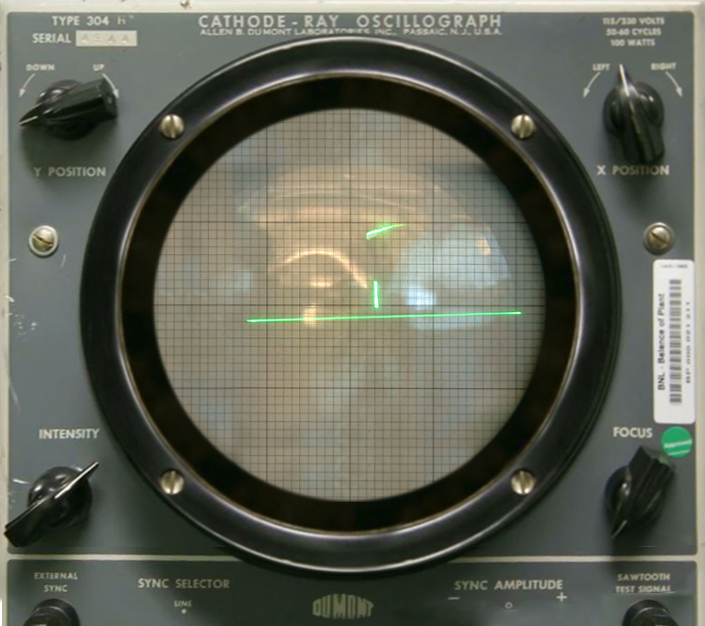
\includegraphics[width=0.8\linewidth]{tennis.jpg}
        \caption{Tennis for Two \parencite{RefWorks:doc:5be168bae4b0273295d7dca5}}\label{tennis}
    \end{subfigure}
    \begin{subfigure}[t]{0.5\textwidth}
        \centering
        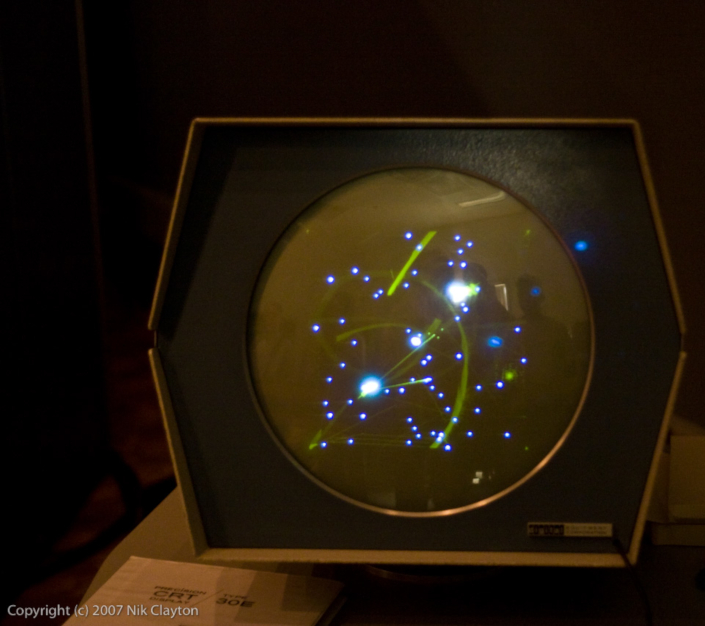
\includegraphics[width=0.8\linewidth]{spacewar.jpg}
        \caption{Spacewar! \parencite{RefWorks:doc:5be162dfe4b0e42e08f77175}}\label{spacewar}
    \end{subfigure}
    \caption{Restauroidut versiot varhaisista videopeleistä.}
\end{figure}

Tennis for Two ja Spacewar! olivat uraa uurtavia videopelejä aikana, jolloin tietokoneet maksoivat satojatuhansia dollareita ja olivat vain vakavaa tieteellistä tai kaupallista käyttöä varten. Higinbothan ja Russell ynnä muut kuitenkin osoittivat, että tietokoneista oli muuhunkin: paitsi että turhanpäiväisten pelien ja sovellusten tekeminen oli hauskaa, sillä oli myös käytännön hyötyä. Spacewar! käytti lähes jokaista PDP-1 -tietokoneen käskyä, joten DEC alkoi käyttää peliä testatessaan ja esitellessään uusien koneidensa toimintaa \parencite{RefWorks:doc:5beac148e4b08968d042364b}. 1970-luvulla videopelejä alettiin kehittää vakavasti ja tuomaan suuren yleisön saataville. 1971 julkaistiin ensimmäiset kolikkopelit Galaxy Game ja Computer Space, jotka molemmat olivat saaneet innoituksensa Spacewar!:sta. Seuraavana vuonna Magnavox julkaisi ensimmäisen kotikonsolin Magnavox Odysseyn. Apple Computer, Commodore ja Tandy julkaisivat vuonna 1977 ensimmäiset massatuotetut kotitietokoneet, joista suosituin oli Apple Computerin pelaamiseen keskittynyt Apple II. \parencitedot{RefWorks:doc:5be15b13e4b05b9281959f24}

Ensimmäiset kolikkopelikoneet, pelikonsolit ja kotitietokoneet käyttivät rasterinäyttöjä, muun muassa sen takia, että vektorinäytöt olivat liian kalliita näihin tarkoituksiin. Larry Rosenthal kuitenkin onnistui rakentamaan tarpeeksi halvan vektorinäytön pelihalleihin, ja vuonna 1977 julkaistiin ensimmäinen vektorinäytöllinen kolikkopeli Space Wars, joka oli Galaxy Gamen ja Computer Spacen tavoin saanut innoituksensa Spacewar!:sta. Vektorinäytön grafiikat olivat huomattavasti terävemmät verrattuna sen aikaisiin pieniresoluutioisiin rasterinäyttöihin, ja tämä saivat pelinkehittäjät innostumaan; syntyivät klassikkopelit Lunar Lander (1979) ja Asteroids (1979), sekä ensimmäiset 3D-pelit Tailgunner (1979) ja Battlezone (1980). Vektorinäyttöjen suosio ei kuitenkaan kestänyt kovin kauan, kun rasterinäytöt kehittyivät vuosikymmenten vaihteessa tarkemmiksi ja värikkäämmiksi. Vuoden 1983 videopelilaman myötä pelihallit eivät enää tilanneet vektoripelejä, eivätkä vektorinäytöt pysyneet rasterinäyttöjen kehityksen perässä. \parencitedot{RefWorks:doc:5be15b13e4b05b9281959f24}

Smith Engineeringin kehittämä, 1982 julkaistu Vectrex on ensimmäinen ja ainoa vektorinäytöllinen kotikonsoli. Vectrex menestyi melko hyvin, mutta sen menestys ei kestänyt kuin reilun vuoden. Videopelilaman takia sen  valmistus lopetettiin jo 1984. Myöhemmin Vectrex on kuitenkin saanut melko merkittävän aseman retropeliharrastajien keskuudessa, ja se on suosittu alusta kotitekoisten pelien (homebrew games) tekemiseen. \parencitedot{RefWorks:doc:5bed604be4b02374b62fe1b5}

\section{Vektorigrafiikan nykytila peleissä}\label{nykypelit}

% - Banner Saga
% - Guacamelee
% - Scribblenauts
% - TF2

Vektorinäyttöjä ei enää ole laajasti saatavilla, mutta monet pelit matkivat niiden tyyliä. Geometry Wars: Retro Evolved (2005) ja Groov (2009) ovat hyviä esimerkkejä moderneista peleistä, jotka ovat saaneet inspiraationsa vanhoista vektoripeleistä. \parencitedot{RefWorks:doc:5be15b13e4b05b9281959f24} On kuitenkin epäselvää, käyttävätkö nämä pelit todellisuudessa vektorigrafiikoita vai bittikarttakuvia, sillä niiden kehittämisestä on hyvin vähän tietoa saatavilla. Sama tiedon puute koskee myös muita pelejä, jotka tyyliltään näyttävät siltä, että voisivat käyttää vektorigrafiikoita. Pelkästään peliä tarkastelemalla on hankala sanoa, käyttääkö se vektori- vai bittikarttagrafiikoita, sillä bittikarttakuvat voivat olla rasteroituja vektorikuvia, näyttäen tietyssä resoluutiossa täysin samalta. Tässä luvussa esitellään joitain videopelejä, jotka käyttävät tiettävästä vektorigrafiikoita ja joiden kehittämisestä löytyy dokumentaatiota.

Yksi näkyvimmin vektorigrafiikoita hyödyntävistä peleistä on Ian Synderin vuonna 2014 julkaisema The Floor is Jelly (ks. kuvio \ref{jelly}). Uniikissa Flashilla ohjelmoidussa tasohyppelypelissä seikkaillaan maailmassa, joka on nimensä mukaisesti tehty hyytelöstä. Hyppiminen ja seiniin törmääminen saa aikaan hytkyvän efektin, joka on mahdollistettu käyttämällä vektorigrafiikoita. \parencitedot{RefWorks:doc:5beea20ce4b06f8a51cf9f11} Blogissaan \textcite{RefWorks:doc:5beec035e4b0463eaf2fd475} kertoo pelimaailman muodostuvan sarjasta pisteitä ja niiden sisään jäävästä väritetystä alueesta. Hyytelöefekti on toteutettu niin, että pisteitä liikutetaan iskun seurauksena aallon tavoin, ja lopulta ne palaavat takaisin lähtöpaikoillensa \parencite{RefWorks:doc:5beec035e4b0463eaf2fd475}. Pelin \parencite{RefWorks:doc:5beea20ce4b06f8a51cf9f11} tiedostojen tarkastelu osoittaa, että pelimaailman lisäksi myös muut pelin grafiikat, kuten pelihahmot ja kasvillisuus, ovat vektorikuvia.

Guacamelee! on DrinkBox Studiosin 2013 julkaisema meksikolaisesta painista inspiroitunut toimintatasohyppelypeli. Guacamelee! on rakennettu DrinkBoxin omalla pelimoottorilla DrinkBox Enginellä, joka on ohjelmoitu C++:lla. Pelihahmojen grafiikat on tehty ja animoitu resoluutioriippumattomasti Flashilla, minkä jälkeen Flash-tiedostot on tuotu DrinkBox Engineen. Vektorikuvat ja -animaatiot mahdollistavat hahmojen skaalaamisen eri kokoisiksi ja 60 fps -animaation. \parencitedot{RefWorks:doc:5bdc818be4b0965708b5a0f0} Hahmoista poiketen pelin tasot ja taustat on tehty kerrostetuista 3D-kappaleista, mikä tuo peliin syvyyden vaikutelmaa \parencite{RefWorks:doc:5beef606e4b03977dc5d4788}.

5Antsin kehittämä ja Rovio Starsin vuonna 2013 julkaisema Tiny Thief on Robin Hood -sävytteinen point-and-click -seikkailupeli Androidille, iOS:lle, Windowsille, OS X:lle ja Wii U:lle \parencites{RefWorks:doc:5bf09463e4b06df665225aeb}{RefWorks:doc:5bf0993ae4b0e21eda418a20}{RefWorks:doc:5bf099d4e4b08f3b86fd2aa3}. 5Antsilla oli kehityksen aikana vaikeuksia Flashilla toteutettujen vektorianimaatioiden ja Adobe AIR -ajoympäristön kanssa. Tiny Thiefin yksi pääelementti oli sen käyttämät 3000 animaatiota, mutta Adobe AIRin rajoitteiden takia vektorigrafiikat eivät toimineet tarpeeksi tehokkaasti joillain laitteilla. Ongelma ratkesi vaihtamalla Adobe AIR Scaleform Mobile SDK:hon, jossa ei ollut samoja rajoitteita. \parencitesdot{RefWorks:doc:5bf09463e4b06df665225aeb}{RefWorks:doc:5bf093b3e4b093d9850ad715} Tiny Thiefin kehittäminen on sittemmin lopetettu ja se on poistettu sovelluskaupoista \parencite{RefWorks:doc:5bf0a115e4b09867bf4e3edb}.

Vaikka 3D-grafiikat pohjautuvatkin vektorigrafiikoihin \parencite{RefWorks:doc:5bdc5224e4b05afcfde5b159}, käytetään niiden teksturoimiseen bittikarttagrafiikoita \parencite{RefWorks:doc:5bf00b76e4b0b28cc7291a34}. Bittikarttagrafiikoiden käyttö on ongelmallista, sillä läheltä tarkasteltaessa niistä tulee epäselviä, tai vaihtoehtoisesti ne pitää tallentaa erittäin suurikokoisina tiedostoina. Tämän ehkäisemiseksi on kehitetty tekniikoita, jotka hyödyntävät vektorigrafiikoita 3D-kappaleiden teksturoinnissa. \parencitedot{RefWorks:doc:5bc4a5cbe4b0af09f17dfdc1} Eräs tällaista tekniikkaa hyödyntävä peli on Valve Corporationin vuonna 2007 julkaisema Team Fortress 2 (ks. kuvio \ref{tf2}). Pelissä esiintyvät tekstuurit on tallennettu etäisyyskenttinä (distance field), jotka ovat bittikarttakuvina koodattuja esityksiä vektorikuvista. Bittikarttakuvia ei esitetä käyttäjälle sellaisenaan, vaan niiden avulla lasketaan kuvan rajat, ja näistä rajoista muodostuvat vektorikuvat esitetään käyttäjälle. Tämä tekniikka mahdollistaa vektorigrafiikoiden esittämisen lähes yhtä tehokkaasti kuin bittikarttagrafiikoiden, mutta se aiheuttaa lievää epätarkkuutta lopulliseen kuvaan. \parencitedot{RefWorks:doc:5bc4a5cbe4b0af09f17dfdc1} 3D-kappaleiden tekstuurien esitys vektorikuvina saattaa tulla erityisen oleellisiksi virtuaalitodellisuutta hyödyntävissä peleissä, joissa venyneiden pikseleiden näkeminen rikkoo immersion tunnetta.

\begin{figure} [!b]
    \begin{subfigure}[t]{0.5\textwidth}
        \centering
        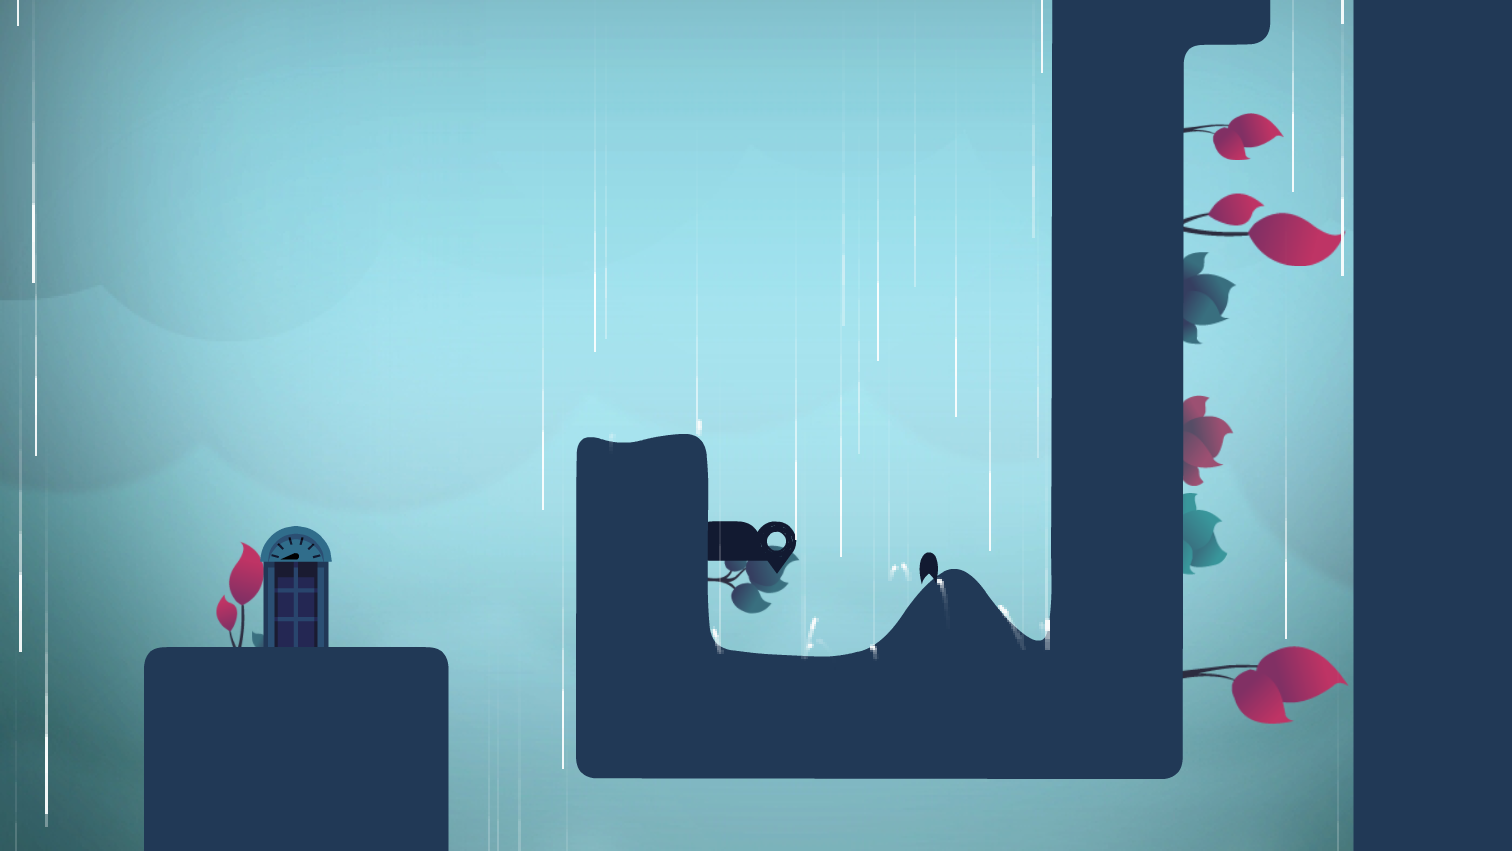
\includegraphics[width=0.8\linewidth]{jelly.png}
        \caption{The Floor is Jelly \parencite{RefWorks:doc:5beea20ce4b06f8a51cf9f11}}\label{jelly}
    \end{subfigure}
    \begin{subfigure}[t]{0.5\textwidth}
        \centering
        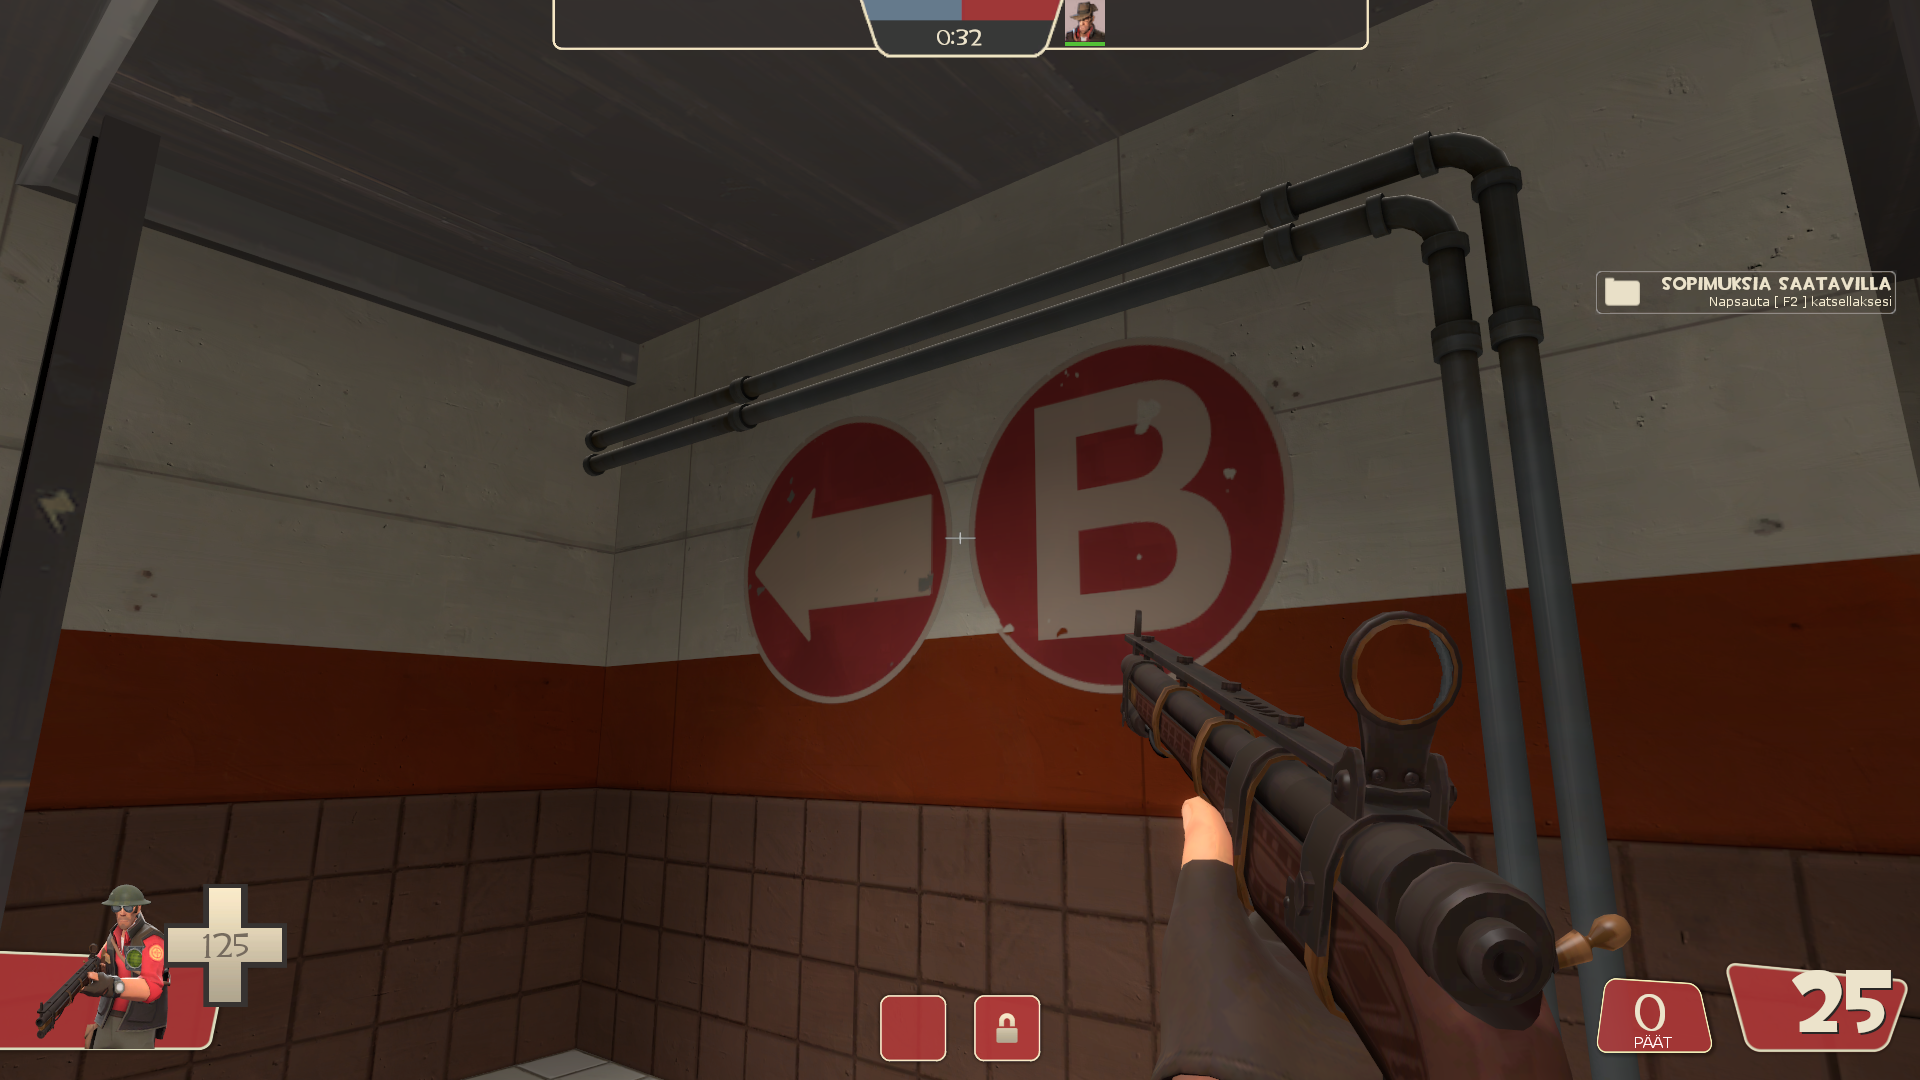
\includegraphics[width=0.8\linewidth]{tf2.png}
        \caption{Team Fortress 2 \parencite{RefWorks:doc:5bf037f1e4b0a014899520eb}}\label{tf2}
    \end{subfigure}
    \caption{Vektorigrafiikoiden käyttö nykyaikaisissa videopeleissä.}
\end{figure}

\section{Ongelmia vektorigrafiikan käytössä}

% - Ei virallista engine tukea
% - "Rajoittunut" tyyli

Vektorigrafiikoiden käytössä on ongelmia, joiden takia ne eivät ole laajasti yleistyneet videopeleissä. Yksi suurimmista ongelmista on suorituskyky. Vaikka koko ajan kehitetään uusia tehokkaampia algoritmeja vektorigrafiikoiden renderöimiseen (esim. \cite{RefWorks:doc:5bc4a5cce4b080e02f7eff1b}), bittikarttagrafiikoiden käyttäminen on huomattavasti tehokkaampaa kuin vektorigrafiikoiden (ks. luku \ref{vertailu}). Tästä syystä kehittäjien on helpompi valita vektorigrafiikoiden sijasta bittikarttagrafiikat peleihinsä. Vektorigrafiikoiden käyttö aiheuttaa kehittäjille ylimääräisiä ongelmia suorituskyvyn kanssa, kuten 5Antsin tapauksessa (ks. luku \ref{nykypelit}).

Usein kehittäjillä ei ole mahdollisuutta vaikuttaa siihen, minkä tyyppisiä grafiikoita he voivat käyttää peleissään. Pelien pohjalla toimii aina pelimoottori, joka määrittelee millaisia ominaisuuksia pelissä voi olla. Pelimoottorista riippuu esimerkiksi millaisia grafiikkatyyppejä tuetaan. TIGAn (\citeyear{RefWorks:doc:5bf14747e4b09ed70a21a7e4}) tekemän tutkimuksen mukaan 53 prosenttia vastanneista pelinkehittäjistä ei käytä itse tekemiään vaan kolmannen osapuolen pelimoottoreita. Unity 3D Engine ja Unreal Engine olivat kyselyn perusteella kaksi eniten käytettyä kolmannen osapuolen pelimoottoria: vastaajista 62 prosenttia käytti Unitya ja 12 prosenttia Unreal Enginea \parencite{RefWorks:doc:5bf14747e4b09ed70a21a7e4}. Unityn ja Unreal Enginen käyttöoppaista selviää, etteivät ne oletusarvoisesti tue vektorigrafiikkatiedostojen käyttöä \parencites{RefWorks:doc:5bf1684be4b045abd3990077}{RefWorks:doc:5bf168ace4b0d4880bbec9aa}, joten monen kehittäjän on tyydyttävä bittikarttagrafiikoihin.

TIGAn kyselyn perusteella kolmannen osapuolen pelimoottorien määrä olisi tulevaisuudessa yhä nousussa. Kyselyyn vastanneista vain 35 prosenttia aikoi jatkossa käyttää itse tekemiään pelimoottoreita. \parencitedot{RefWorks:doc:5bf14747e4b09ed70a21a7e4} Tällainen kehitys siirtää vastuun tuetuista grafiikkatyypeistä yhä enemmän pois yksittäisten pelikehittäjien käsistä pelimoottorien kehittäjien käsiin. Onkin havaittavissa, että kiinnostus vektorigrafiikoita kohtaan olisi kasvamassa sekä pelimoottoreiden käyttäjien että niiden kehittäjien keskuudessa. Unityyn ja Unreal Engineen on kumpaankin saatavilla epävirallisia SVG-tiedostoja tukevia lisäosia, jotka eivät kuitenkaan tue kaikkia tiedoston ominaisuuksia \parencites{RefWorks:doc:5bf1712ce4b0efa59d30f4f7}{RefWorks:doc:5bf17193e4b09ed70a21ac25}. Lisäksi heinäkuussa 2018 julkaistuun Unityn versioon 2018.2 sisältyy testiversio SVG-paketista, jonka avulla voidaan käyttää SVG-tiedostoja sekä luoda ja muokata vektorikuvia ohjelmallisesti. Unity ei renderöi SVG-kuvia perinteisesti, vaan pilkkoo kuvan automaattisesti sopivaksi määräksi helposti renderöitäviä kolmioita. \parencitedot{RefWorks:doc:5c0153b7e4b0d07d385793b5}

Bittikarttagrafiikoiden käyttö vektorigrafiikkojen sijasta voi myös olla taiteellinen valinta. Vektorigrafiikat sopivat hyvin selkeiden muotojen esittämiseen, mutta tavoiteltaessa esimerkiksi realistista tyyliä bittikarttakuvat ovat parempi vaihtoehto \parencite{RefWorks:doc:5bdc5224e4b05afcfde5b159}. Realistisen tyylisten tai muuten monimutkaisten vektorikuvien tiedostokoko voi olla valtavan suuri \parencite{RefWorks:doc:5bdf4af9e4b0f02deeb8a48a}, ja niiden renderöimiseen tarvittava laskentateho kohtuuton. Monimutkaisen grafiikan tapauksessa vektorigrafiikoiden käyttö ei ole suositeltavaa \parencite{RefWorks:doc:5bdf4af9e4b0f02deeb8a48a}. \textcite{RefWorks:doc:5bf1b71ae4b0bdd1f93c0e3c} -keskustelufoorumilla käydyn keskustelun perusteella monien mielestä vektorigrafiikat ovat yksinkertaisesti rumia, ja ne yhdistetään huonolaatuisiin ilmaisiin nettipeleihin, jotka on tehty Flashilla ja käyttävät vektorigrafiikoita. Vektorigrafiikkoihin tuntuukin liittyvän monia harhaluuloja ja ennakkoluuloja.

Vektorikuvien tekemisen työnkulku on erilainen kuin bittikarttakuvien, sillä piirtämisen ja maalaamisen sijasta määritelläänkin pisteiden sijainteja ja ominaisuuksia. Tästä syystä vektorigrafiikoiden tekeminen voi olla vaikeaa niille, jotka ovat tottuneet tekemään videopeligrafiikoita bittikarttagrafiikkoina. Ne puolestaan, jotka ovat tottuneet tekemään vektorigrafiikoita, ovat usein tottuneet tekemään graafisia esityksiä, kuten logoja, pelihahmojen sijasta. Nykyaikaiset vektorigrafiikkaohjelmat, kuten Adobe Systemsin (\citeyear{RefWorks:doc:5bf1ca5ee4b03fd0c4891238}) Adobe Illustrator ovat pyrkineet madaltamaan vektorigrafiikoiden tekemisen kynnystä mahdollisimman paljon. Adobe Illustrator tarjoaa monia bittikarttagrafiikkaohjelmista tuttuja ominaisuuksia, kuten erilaisia siveltimiä, joiden avulla vektorikuvaan voi lisätä viivoja ikään kuin maalaten. \parencitedot{RefWorks:doc:5bf1ca5ee4b03fd0c4891238}

\chapter{Yhteenveto}

% - Tarvitaan esimerkki proto

Vektorigrafiikoiden käytön videopeleissä voi jakaa kahteen aikakauteen: ennen ja jälkeen vuoden 1983 videopelilaman. Ennen lamaa kukoistivat niin sanotut oikeat vektoripelit, eli pelit, joita pelattiin vektorinäytöillä. Laman jälkeen siirryttiin käyttämään rasterinäyttöjä eivätkä vektorigrafiikat enää täyttäneet yleisön vaatimuksia. Lähes kaikki pelit 80-luvulta lähtien käyttävätkin bittikarttagrafiikoita. Vektorigrafiikoiden renderöinti rasterinäytölle sopivaksi vaatii paljon laskentatehoa, jota varsinkaan 80-luvun tietokoneissa ei ollut. Teknologian kehittymisen myötä vektorigrafiikoita on voitu hyödyntää paremmin, mutta vieläkään niistä ei ole tullut yleisesti käytettyjä videopeleissä. Edes viimeisen kymmenen vuoden ajalta on vaikea löytää vektorigrafiikoita käyttäviä pelejä, mikä on osaltaan hankaloittanut tämän tutkielman tekoa.

Tehokkaampien algoritmien ja laitteistojen kehittäminen antaa mahdollisuuden tehdä pelejä, joissa on enemmän ja monimutkaisempia vektorikuvia. Tekniikan kehittyminen parantaa kehittäjien kykyä käyttää peleissään vektorikuvia graafisesta tyylistä riippumatta. Olemassa olevien ominaisuuksien parantamisen lisäksi vektorigrafiikoihin kehitetään myös uusia ominaisuuksia. Esimerkiksi \textcite{RefWorks:doc:5bfd0d4de4b0bf300b66d3fe} esittävät täysin uudenlaista vektorigrafiikkaelementtiä, diffuusiokäyrää. Käyrien välinen alue täytetään käyrien värejä vastaavilla liukuväreillä, ja näin saadaan luotua erittäin monimutkaisia vektorikuvia vain muutamalla käyrällä. \parencitedot{RefWorks:doc:5bfd0d4de4b0bf300b66d3fe} Uudet teknologiat mahdollistavat vektorigrafiikoiden käytön sellaisissa graafisissa tyyleissä, joissa ne eivät ole ennen toimineet.

Teknisesti on siis täysin mahdollista käyttää vektorigrafiikoita videopeleissä, mutta käytännössä siinä on vielä monia ongelmia. Puuttuvan pelimoottorituen ja virheellisten ennakkoluulojen takia käytetään mieluummin bittikarttagrafiikat harkitsemattakaan vektorigrafiikoita. Unityn SVG-paketin olemassaolo kuitenkin kertoo vektorigrafiikoille olevan niin paljon kysyntää, että tällaisen paketin tekeminen koetaan liiketoiminnallisesti kannattavana. Vektorifiikoiden näkyvyyden lisääntyminen pelinkehittäjien keskuudessa lisää vektorigrafiikoiden käyttöä ja samalla huomataan, etteivät vektorigrafiikat automaattisesti tarkoita alkeellisia ja yksinkertaisia grafiikoita. Kehittyneiden teknologioiden ansiosta on mahdollista tehdä edistyneitä ja monimuotoisia vektorikuvia, joita voi silti renderöidä reaaliaikaisesti.

Aiheeseen liittyvä tieteellinen tutkimus on vähäistä ja tutkielman myötä herää monia tutkimuskysymyksiä tulevaisuuteen. Olisi mielenkiintoista selvittää vektorigrafiikoiden käytön osuus kaikissa videopeleissä. Entä miten vektorigrafiikoiden käyttö vaikuttaa pelin kehittämiseen käytettyyn aikaan ja budjettiin, tai lopullisen pelin tiedostokokoon ja suorituskykyyn? Tätä voitaisiin jatkossa tutkia esimerkiksi toteuttamalla samanlainen peli käyttäen sekä bittikarttagrafiikoita että vektorigrafiikoita ja vertailemalla käytettyjä työmääriä ja pelien suorituskykyjä. Tieteellinen tutkimus voisi tuoda lisää näkyvyyttä vektorigrafiikoiden käytölle videopeleissä ja mahdollisesti vähentää niihin liittyviä ennakkoluuloja.

% Tieteellisen tutmikuksen avulla voitaisiin tehdä vektorigrafiikoita yhe edelleen näkyvämmäksi ja mrtaaa ennakkoluuloja ja siten tuoda lisää mahdollisuuksia pelinkehittämiseen.

\printbibliography

\end{document}